\documentclass[conference]{IEEEtran}
\IEEEoverridecommandlockouts
% The preceding line is only needed to identify funding in the first footnote. If that is unneeded, please comment it out.
\usepackage{cite}
\usepackage{amsmath,amssymb,amsfonts}
\usepackage{algorithmic}
\usepackage{graphicx}
\graphicspath{{../images/}}
\usepackage{textcomp}
\usepackage{xcolor}
\usepackage{svg}
\usepackage{listings}
\usepackage{tcolorbox}  % For rounded boxes
\usepackage{courier}   
\usepackage{hyperref}
\hypersetup{
    colorlinks=true,
    linkcolor=blue,
    filecolor=magenta,      
    % urlcolor=cyan,
    % pdftitle={Overleaf Example},
    % pdfpagemode=FullScreen,
    }
% \usepackage{algorithm}
\usepackage[ruled,vlined]{algorithm2e} %linesnumbered, Use algorithm2e for better line numbering
\usepackage{algpseudocode}
\usepackage{enumitem}
\def\BibTeX{{\rm B\kern-.05em{\sc i\kern-.025em b}\kern-.08em
    T\kern-.1667em\lower.7ex\hbox{E}\kern-.125emX}}
\begin{document}

\title{Padding Oracle Attack on CBC Mode\\
{\footnotesize \textsuperscript{*}Report for \textit{Indian Institute of Technology Bombay} - CS 409M: Introduction to Cryptography ({\it Autumn 2024})}
% \thanks{Identify applicable funding agency here. If none, delete this.}
}

\author{\IEEEauthorblockN{Harsh Sanjay Roniyar}% 1\textsuperscript{st} Given Name Surname}
\IEEEauthorblockA{\textit{Department of Electrical Engineering} \\
\textit{Indian Institute of Technology Bombay}\\
Mumbai, India \\
22b3942@iitb.ac.in}
\and
\IEEEauthorblockN{Swarup Patil}% 2\textsuperscript{nd} Given Name Surname}
\IEEEauthorblockA{\textit{Department of Electrical Engineering} \\
\textit{Indian Institute of Technology Bombay}\\
Mumbai, India \\
22b3953@iitb.ac.in}
}

\maketitle

\begin{abstract}
This report highlights and demonstrates a padding oracle attack on CBC (Cipher Block Chaining) mode.
The attack exploits the fact that after decryption, the padding on the last block is validated. The attacker sends modified ciphertexts to the padding oracle and observes whether the padding is valid. Through repeated guesses and error analysis, the attacker can determine the plaintext without knowing the decryption key.

% This document is a model and instructions for \LaTeX.
% This and the IEEEtran.cls file define the components of your paper [title, text, heads, etc.]. *CRITICAL: Do Not Use Symbols, Special Characters, Footnotes, 
% or Math in Paper Title or Abstract.
\end{abstract}

\begin{IEEEkeywords}
cryptography, oracle, padding, cipher block chaining
% component, formatting, style, styling, insert
\end{IEEEkeywords}

\section{Introduction}
A padding oracle attack in cryptography exploits the process of padding validation to decrypt ciphertext. Since variable-length plaintext messages often need padding to align with the cryptographic algorithm, the attack takes advantage of a ``padding oracle" that reveals whether the padding in a message is correct. This feedback, whether explicitly provided or leaked through side-channels, enables the attacker to decrypt the message.

\section{Background}
The first well-known padding oracle attack was Bleichenbacher's 1998 attack on RSA with PKCS \#1 v1.5 padding. The term ``padding oracle" became popular after Serge Vaudenay's 2002 attack on CBC mode decryption in symmetric block ciphers. Both attacks are still relevant today. In symmetric cryptography, padding oracle attacks exploit CBC mode, where information about padding can help attackers decrypt or encrypt messages using the oracle's key, without knowing the encryption key. Vaudenay's attack is more efficient than Bleichenbacher's, and while CBC was widely used in SSL and TLS, newer timing attacks have revived the issue. TLS 1.2 introduced authenticated encryption modes to mitigate these risks.

% \section{Problem}

\section{The XOR (\textit{Exclusive-OR})}
The XOR is a two-bit operator that compares corresponding bits in two binary inputs. It outputs 1 if the number of input bits that are 1 is odd and outputs 0 if it is even. The operation is mathematically equivalent to addition \texttt{mod} 2.

$$\left(a \oplus b = c\right) \Leftrightarrow \left(b \oplus c = a\right) \Leftrightarrow \left(c \oplus a = b\right)$$

Additionally, XOR is cyclic when applied to three bit strings; this means XORing the same three bit strings in any order results in the same output, and applying XOR repeatedly to the same bit strings will eventually return to the original input.


\section{Cipher Block Chaining (CBC) Mode}
\textbf{Cipher Block Chaining (CBC)} is a mode of operation for block ciphers where data is encrypted in blocks, with each block XORed with the previous ciphertext block, using an initialization vector (IV) and a single encryption key, enabling secure encryption of large amounts of plaintext. Therefore, CBC mode enhances the security of block ciphers by introducing randomness and interdependency between ciphertext blocks. 

\subsection{Encryption in CBC Mode}
In CBC, each plaintext block is XORed with the ciphertext of the previous block before being encrypted. Mathematically, this can be described as:
\[
C_1 = E(P_1 \oplus IV)
\]
\[
C_n = E(P_n \oplus C_{n-1}) \quad \text{for } n > 1
\]
where \(P_n\) is the plaintext block, \(C_n\) is the ciphertext block, \(E()\) is the encryption function, and \(IV\) is the initialization vector, which is typically a random value.

\begin{figure}[!htb]
    \centering
    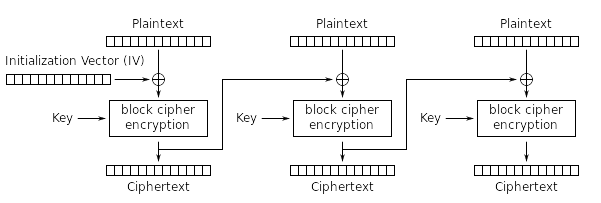
\includegraphics[width=0.5\textwidth]{CBC_encryption.png}
    \caption{Cipher Block Chaining (CBC) Mode Encryption}
    \label{fig:enter-label}
\end{figure}

\subsection{Decryption in CBC Mode}
Decryption in CBC mode reverses the process. The ciphertext is decrypted, and then the result is XORed with the previous ciphertext block to recover the plaintext:
\[
P_1 = D(C_1) \oplus IV
\]
\[
P_n = D(C_n) \oplus C_{n-1} \quad \text{for } n > 1
\]
where \(D()\) is the decryption function. 

This chaining process ensures that even small changes in the ciphertext propagate through all subsequent blocks, enhancing security. However, this dependency also makes CBC vulnerable to Padding Oracle Attacks.

\begin{figure}[!htb]
    \centering
    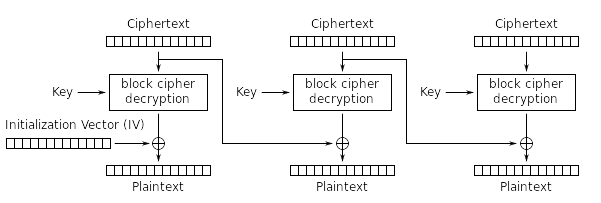
\includegraphics[width=0.5\textwidth]{CBC_decryption.png}
    \caption{Cipher Block Chaining (CBC) Mode Decryption}
    \label{fig:enter-label}
\end{figure}

\section{Block Ciphers and Padding}
\subsection{Block Ciphers}
A block cipher is a deterministic algorithm that operates on fixed-length groups of bits, called blocks. Examples of block cipher algorithms include {\bf AES} (128-bit blocks) and {\bf DES} (64-bit blocks). 

\subsection{Padding Scheme}
The {\bf PKCS \#7} padding scheme is a method used in cryptographic encryption to handle data that doesn’t fit the exact block size of encryption algorithms like AES, which require inputs to be divided into fixed-size blocks, typically 16 bytes.

The number of padding bytes added is equal to the difference between the block size and the length of the final block. Each padding byte contains a value indicating how many bytes were added. For example, if 6 bytes are needed, each byte will have the value 06 in hexadecimal. Even when the plaintext fits the block size exactly, a full block of padding is still added, with each byte representing the block size.

When decrypting, the value of the last byte indicates how many padding bytes were used, and these bytes are then removed.This padding ensures smooth encryption and is used in secure communication protocols and encryption standards.

\begin{figure}[!htb]
    \centering
    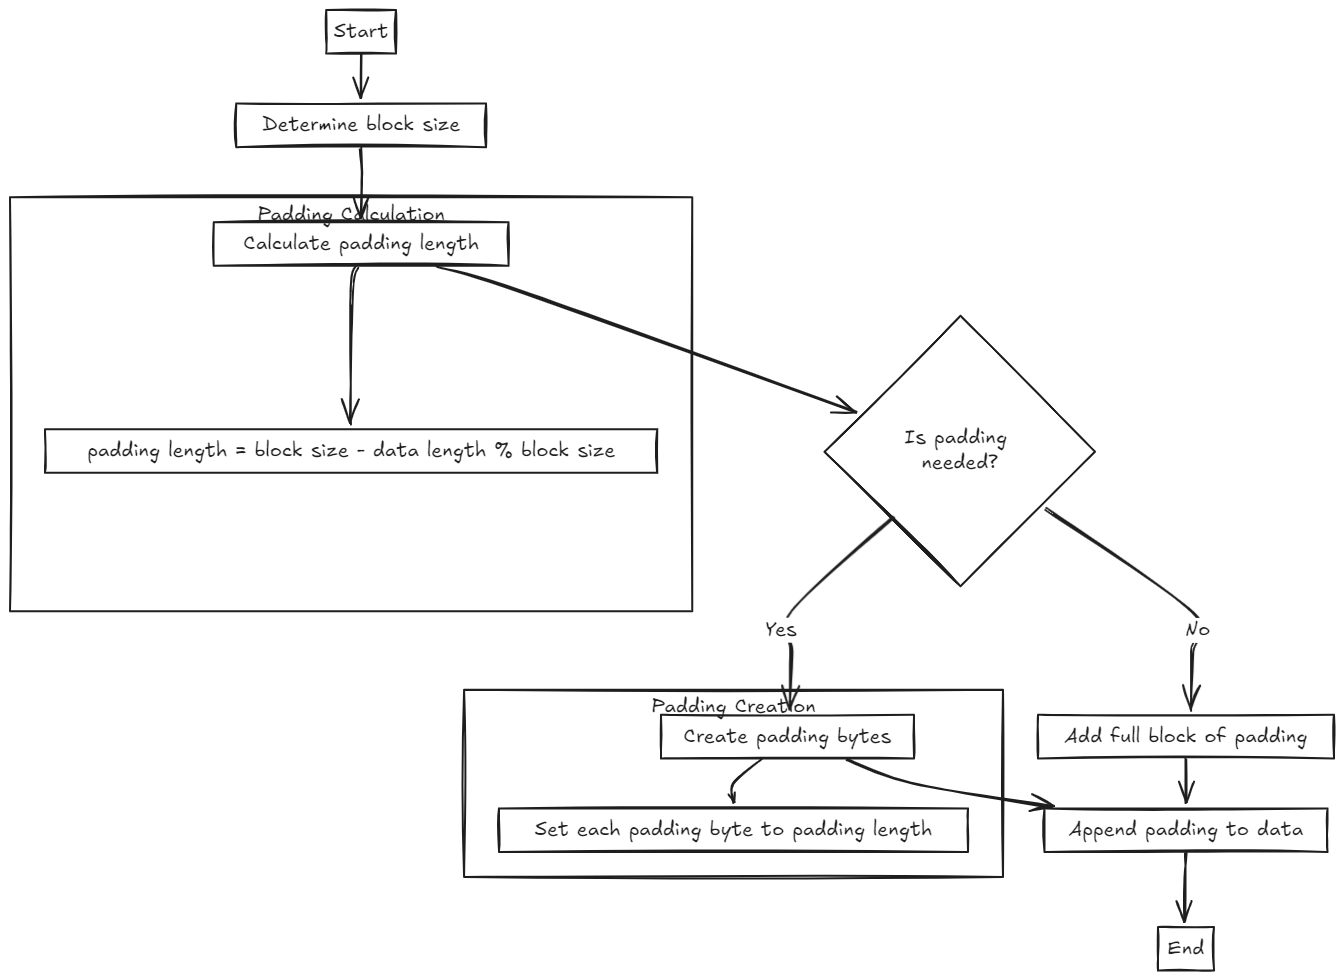
\includegraphics[width=\linewidth]{padding.png}
    \caption{Illustration of the PKCS \#7 Padding Scheme}
    \label{fig:padding-scheme}
\end{figure}
% For a block size of 16 bytes, PKCS \#7 padding works as follows:
% \[
% \text{``ABCDEFGHIJ"} \rightarrow \text{``ABCDEFGHIJ}\backslash\text{06}\backslash\text{06}\backslash\text{06}\backslash\text{06}\backslash\text{06}\backslash\text{06}"
% \]

% If the message perfectly fits the block size, an entire block of padding is added.
If a string is a multiple of the block size, an extra block of padding is added to distinguish cases like ``$\text{ABC}\ldots\text{O}\backslash \text{x}01$" (where ``$\backslash \text{x}01$" is part of the string) from ``$\text{ABC}\ldots\text{O}$" with padding.
Padding is crucial in identifying the end of a message and ensuring that block ciphers process complete blocks.

\section{The Oracle}
A Padding Oracle functions as a blackbox that receives an encrypted message as input. Upon receiving the message, the oracle internally decrypts it using a predefined cryptographic key. After decryption, the oracle checks whether the decrypted message conforms to the expected padding scheme, such as PKCS \#7 or another padding standard. Based on this validation, the oracle responds with a boolean outcome: it returns `true' if the message has valid padding and `false' if the padding is incorrect. 

This seemingly simple feedback can be exploited by attackers to iteratively modify the ciphertext and extract information about the plaintext or the decryption key, making padding oracles a critical vulnerability in improperly secured systems.
\begin{figure}[!htb]
    \centering
    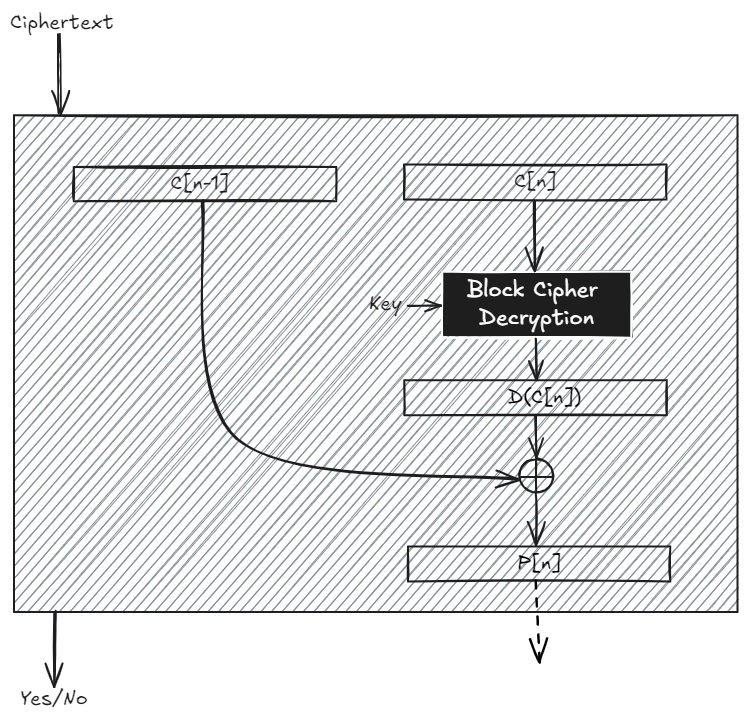
\includegraphics[width=0.8\linewidth]{oracle.png}
    \caption{The Oracle Block}
    \label{fig:oracle}
\end{figure}

\section{Attack Algorithm}

In this section, we present a systematic attack algorithm that leverages vulnerabilities in the padding scheme to recover plaintext from ciphertext in the CBC mode of operation. 

The attacker exploits this oracle by crafting specific ciphertext modifications to deduce the plaintext byte by byte. 

The algorithm proceeds as follows:
\begin{enumerate}
    \item The attacker intercepts the ciphertext and divides it into individual blocks. Let \(C = (C_1, C_2, \dots, C_n)\) be the intercepted ciphertext.
    \item Starting from the last block, the attacker generates a custom block \(C'\) and concatenates it with \(C_n\), sending the modified ciphertext \((C' || C_n)\) to the oracle.
    \item The oracle decrypts the message and checks the padding. If the padding is valid, the attacker knows that the last byte of the plaintext has the correct padding byte (e.g., \(\backslash \text{x}01\)).
    \item By modifying the last byte of \(C'\) and resubmitting, the attacker can iteratively guess the correct value for each byte of the plaintext.
\end{enumerate}

\subsection{Decrypting the Last Block}

In this subsection, we outline the steps the attacker follows to decrypt the last block of the intercepted ciphertext, denoted as \(C_n\). The process involves crafting a custom ciphertext block $C'$ that, when appended to $C_n$, can be sent to the padding oracle to validate the padding and thereby infer the values of the plaintext bytes in $C_n$.

% The attacker focuses on decrypting the last ciphertext block \(C_n\). 
The process is as follows:
\begin{enumerate}
    \item The attacker creates a new ciphertext block \(C'\). Typically, a block of zeroes is used:
    \[
    C' = \text{0x000}\ldots\text{0}
    \]
    \item Form a new ciphertext by concatenating \(C'\) and \(C_n\):
    \[
    C' || C_n
    \]
    \item The attacker sends \(C' || C_n\) to the padding oracle for decryption.
\end{enumerate}

\subsection{Understanding the Decryption}

This subsection delves into the mechanics of how the padding oracle decrypts the modified ciphertext \( C' \, || \, C_n \). The decryption of \( C' \) is not relevant to the attack, but the plaintext from \( C_n \) contains vital information the attacker aims to exploit. Understanding this process is key to isolating and calculating the plaintext bytes.

When the oracle decrypts \(C' || C_n\), it performs the following operations:
\[
P'_1 = D(C') \oplus IV
\]
\[
P'_2 = D(C_n) \oplus C'
\]
where:
\begin{itemize}
    \item \(P'_1\) is the plaintext block resulting from decrypting \(C'\).
    \item \(P'_2\) is the plaintext block resulting from decrypting \(C_n\) with \(C'\).
\end{itemize}

Since \(P'_1\) is irrelevant (garbage), the focus is on \(P'_2\):
\[
P'_2 = D(C_n) \oplus C'
\]
Using the encryption definition \(C_n = E(P_n \oplus C_{n-1})\), we substitute:
\[
P'_2 = D(E(P_n \oplus C_{n-1})) \oplus C' = P_n \oplus C_{n-1} \oplus C'
\]
Thus:
\[
P'_2 = P_n \oplus C_{n-1} \oplus C'
\]

The challenge we face is the presence of two unknown values: \( P'_{2} \) and \( P_{n} \). Since a formula with two unknowns cannot be resolved directly, we can leverage the padding oracle to extract additional information. By manipulating \( C' \) and analyzing the oracle's responses, the attacker can effectively deduce the value of \( P_{n} \).

\subsection{Exploiting the Padding Oracle}

The attacker aims to manipulate \(C'\) such that the padding in \(P'_2\) is valid. Specifically, the oracle reveals whether the padding is correct or not, allowing the attacker to infer information about \(P_n\).

\subsubsection{Determining the Last Byte \(P_n[k]\)}
In this step, we focus on isolating and computing the last byte of the plaintext block \(P_n\). By systematically varying \(C'[k]\) and submitting the modified ciphertext to the oracle, the attacker can determine which byte value produces valid padding. This demonstrates the practical application of XOR properties, allowing the extraction of individual bytes from the plaintext.

To illustrate, consider the last byte, denoted as \(k\):
\[
P'_2[k] = P_n[k] \oplus C_{n-1}[k] \oplus C'[k]
\]
For valid padding to be recognized, the value \( P'_{2}[K] \) can represent valid padding bytes such as ``$\backslash\text{x}01$", "$\backslash\text{x}02$", or any other permissible padding value. However, we will specifically enforce the condition that \( P'_{2}[K] \) must equal ``$\backslash\text{x}01$".
\[
1 = P_n[k] \oplus C_{n-1}[k] \oplus C'[k]
\]

At this point, we have identified the following variables: \( P'_{2}[K] \), the valid padding value ``$\backslash \text{x01}$"; \( P_{n}[K] \), the unknown last byte of the plaintext; \( C_{n-1}[K] \), the known last byte of the previous ciphertext block; and \( C'{[K]} \), the controlled byte we modified for valid padding. 

With these three known variables, we can reformulate the equation, leveraging the commutative property of the XOR operation to rearrange them as necessary.



Solving for \(P_n[k]\), we get:
\[
P_n[k] = 1 \oplus C_{n-1}[k] \oplus C'[k]
\]

The execution of the attack proceeds by varying \(C'[k]\) across all byte values from 0 to 255. For each value, the attacker constructs the modified ciphertext \(C' || C_n\) and submits it to the oracle. The oracle's response reveals the specific value of \(C'[k]\) that results in valid padding. Once the valid padding is found, the corresponding plaintext byte \(P_n[k]\) can be computed using the above equation, allowing the attacker to extract the plaintext byte by byte.

\newpage
\subsubsection{Determining Earlier Bytes \(P_n[k-i]\)}
We extend the attack strategy to uncover the bytes preceding the last byte of the plaintext block. By adjusting the custom ciphertext \(C'\) to enforce valid padding conditions for these earlier byte positions, the attacker can iteratively deduce the complete plaintext block. This section illustrates how the same principles applied to determine the last byte can be adapted to extract earlier bytes.

\textit{{\bf Example}: Determining \(P_n[k-1]\)}

First, we need to assign \( C'{[k]} \) an appropriate value to ensure that \( P'{[k]} = 2 \). The reason for selecting the value 2 is that we aim to ascertain the second-to-last byte of \( P'_{n} \). By setting the last byte to 2, we can systematically vary \( C'{[k-1]} \) through all possible values until we no longer encounter padding errors. This successful configuration will confirm that \( P'_{n} \) concludes with the byte sequence ``$\backslash \text{x02}\backslash \text{x02}$”.

\[
P'_2[k] = P_n[k] \oplus C_{n-1}[k] \oplus C'[k] = 2
\]
\[
2 = P_n[k] \oplus C_{n-1}[k] \oplus C'[k]
\]
Solving for \(P_n[k-1]\):
\[
P_n[k-1] = 2 \oplus C_{n-1}[k-1] \oplus C'[k-1]
\]

\subsection{Iterative Decryption}
The attacker employs an iterative process to decrypt the entire plaintext block \(P_n\) byte by byte, starting from the last byte and moving to the first. Each iteration focuses on establishing valid padding conditions and utilizing the oracle's responses to systematically reveal the values of all bytes in the block. 

For each byte position \(i\) from \(k\) down to 1:
    \begin{enumerate}
        \item Set padding value to \(i\) (i.e., \texttt{\textbackslash x$i$}).
        \item Adjust corresponding bytes in \(C'\) to satisfy the padding condition.
        \item Use the oracle to validate padding and deduce the plaintext byte \(P_n[i]\).
    \end{enumerate}

Similarly, just as we can recover the last plaintext block \(P_n\), we can also decrypt the preceding blocks \(P_{n-1}, P_{n-2}, \dots\). Each block can be decrypted independently, provided the ciphertext of the preceding block is available.

This brings us to the first plaintext block \( P_1 \). As previously noted, \( P_1 \) is determined by the equation:
\[
P_1 = D(C_1) \oplus \text{IV}
\]
where:
\begin{itemize}
    \item \( P_1 \) represents the first plaintext block.
    \item \( C_1 \) is the first ciphertext block.
\end{itemize}

In this case, the initialization vector (IV) acts as the previous ciphertext block for \( P_1 \), in the same way \( C_{n-1} \) does for other blocks.

After successfully decrypting all blocks of ciphertext using the padding oracle attack, we obtain the complete plaintext \( P \). Once all the plaintext blocks are recovered, the padding added during encryption is removed by checking the last byte, which indicates the length of the padding. By stripping off the padding, we finally retrieve the original message. 

% This process highlights the vulnerability in padding schemes, emphasizing the need for secure padding validation and encryption methods to prevent such attacks.

\section{Implementation}

The attack algorithm was implemented in Python using AES-128 Symmetric Key Encryption. The structure of the overall code is described by the pseudocode below.

\RestyleAlgo{ruled}
\begin{algorithm}
\caption{Padding Oracle Attack}
\KwIn{Ciphertext \(C\), Oracle \(O\)}
\KwOut{Plaintext \(P\)}

\For{block \(i \leftarrow n \text{ to } 1\)}{
    Initialize empty plaintext block \(P_i\)\;
    \For{byte \(j \leftarrow \text{size(block)} \text{ to } 1\)}{
        \For{each possible byte value \(v \leftarrow 0 \text{ to } 255\)}{
            Construct modified ciphertext \(C'\)\;
            Send \(C'\) to oracle \(O\)\;
            \If{oracle returns \texttt{True}}{
                Set \(P_i[j] \)\;
                Break loop\;
            }
        }
    }
}
\Return \(P\)\;
\end{algorithm}

The complete implementation can be found in the GitHub repository linked at the end of this report.

\section{Result}

The padding oracle attack works within a complexity of $\mathcal{O}$(NbW) in order to decrypt the message where W is the number of possible words (typically W = 256), N is the number of blocks, and b is the block size.

After completing the implementation code, we conducted tests using custom inputs to execute the padding oracle attack. We then verified that the decrypted output matched the original input. 
\lstset{
    basicstyle=\ttfamily\footnotesize,  % Custom font style and size
    keywordstyle=\color{blue}\bfseries, % Custom keyword style
    commentstyle=\color{gray},          % Custom comment style
    morekeywords={unsigned, char, int, void}, % Specify keywords
    backgroundcolor=\color{gray!10},    % Light gray background for code
    columns=fullflexible,
    keepspaces=true,
    breaklines=true,
    language=C++,                      % Specify the language
    % style=Matlab-Pyglike,
    escapeinside={(*@}{@*)}
}

% Rounded box style
\tcbset{
    colframe=black!75!white,    % Border color
    colback=gray!10,            % Background color
    boxrule=0.5pt,              % Border thickness
    arc=6pt,                    % Rounded corners
    outer arc=6pt,
    top=5pt,                    % Padding
    bottom=5pt,
    left=5pt,
    right=5pt,
    fonttitle=\bfseries,        % Bold title font
}

\begin{tcolorbox}[title={Attack Test Output}]
\begin{lstlisting}
------------------------------------
Testing : b'Attack at dawn' OF LENGTH 14
The encrypted message is : b"Xi\x95RA\xb3\x97v,\xb9\x91\xe3;\xfa'\xd5n\xfcLT@\xb2\xa8\xf2\xda}\xceqM\xfff\xda"
The decrypted message (with padding) is : bytearray(b'Attack at dawn\x02\x02')
------------------------------------
Assertion passed!
------------------------------------
------------------------------------
Testing : b'' OF LENGTH 0
The encrypted message is : b'\xcd\xca\xbdIB\xe9\xde\xfd\xda\xb7#A-X\xe9!\x9c\xa6\x98f\xab\xb1\x07\xbe\n\x9928\x8c\xdc*\xe7'
The decrypted message (with padding) is : bytearray(b'\x10\x10\x10\x10\x10\x10\x10\x10\x10\x10\x10\x10\x10\x10\x10\x10')
------------------------------------
Assertion passed!
------------------------------------
------------------------------------
\end{lstlisting}
\end{tcolorbox}


\section{Improvement}

The integration of authentication into the CBC-PAD scheme was initially deemed unnecessary, but Wagner’s attack underscored the critical need for such measures in cryptographic protocols. In response, a comprehensive scheme has been proposed that simultaneously ensures authentication and confidentiality by applying both mechanisms to the padded plaintext.

The process commences with padding the cleartext, which is then authenticated and encrypted before transmission. During decryption, the first step involves verifying the authenticity of the received data, followed by padding validation to ensure integrity. Once these checks are complete, the cleartext can be accurately extracted.

It is important to differentiate between cleartext—the original message—and plaintext, the data input into the encryption algorithm. While Krawczyk's authenticate-then-encrypt method has shown promise, it remains susceptible to side-channel attacks, indicating a need for further scrutiny. Although formal proofs of the proposed scheme's security are lacking, it is expected to provide a robust defense against various threats, thereby enhancing the CBC-PAD framework's overall security.


\section*{Acknowledgment}

We express our sincere gratitude to Prof. Sruthi Sekar for the opportunity to explore the topic of Padding Oracle Attack on CBC Mode through the Chalk and Talk initiative in CS 409M. This experience allowed us to deepen our understanding of this attack methodology, enhancing our exploration of cryptographic vulnerabilities. Additionally, collaborating on the presentation enabled us to effectively convey our findings and insights.

\begin{thebibliography}{00}
\bibitem{b0} \href{https://github.com/hsr-22/PaddingOracleAttack-CBC}{Our code repository of attack implementation}
\bibitem{b1} \href{https://doi.org/10.1007/3-540-46035-7_35}{Vaudenay, S. (2002). Security Flaws Induced by CBC Padding — Applications to SSL, IPSEC, WTLS....}
\bibitem{b2} \href{https://www.skullsecurity.org/2013/padding-oracle-attacks-in-depth}{Padding oracle attacks: in depth by SkullSecurity}
\bibitem{b3} \href{https://www.cs.umd.edu/~jkatz/imc2.html}{Katz and Lindell Book(2nd Edition) - Section 3.7.2}
\bibitem{b4} \href{https://en.wikipedia.org/wiki/Padding_oracle_attack}{Wikipedia - Padding Oracle Attack}
\bibitem{b5} \href{https://www.youtube.com/watch?v=4EgD4PEatA8}{CS2107 Padding Oracle Attack}

\end{thebibliography}

\end{document}